\section{Intro}

\mult{2}

\begin{definition}{Definition of Machine Learning}\\
    Machine Learning (ML) is a branch of artificial intelligence (AI) devoted to developing and understanding methods that "learn", i.e., that leverage data to make predictions or decisions without being explicitly programmed to do so.\\
    $\Rightarrow$ Study of algorithms and statistical models without using explicit instructions, relying on patterns and inference instead
\end{definition}

\begin{concept}{Purpose of Machine Learning}\\
The computational methods in ML are used to discover patterns in data and/or derive a corresponding generating process to:
\begin{itemize}
    \item Gain insights and predict events
    \item Provide a quantitative basis for decisions (actionable insights)
    \item Influence the underlying process of the data
\end{itemize}
$\Rightarrow$ Branch of AI devoted to developing and understanding methods that "learn", i.e. that leverage fata to make predictions or decisions (act like humans) without being explicity programmed to do so
\end{concept}

\begin{definition}{What's behind the Magic?} \\
    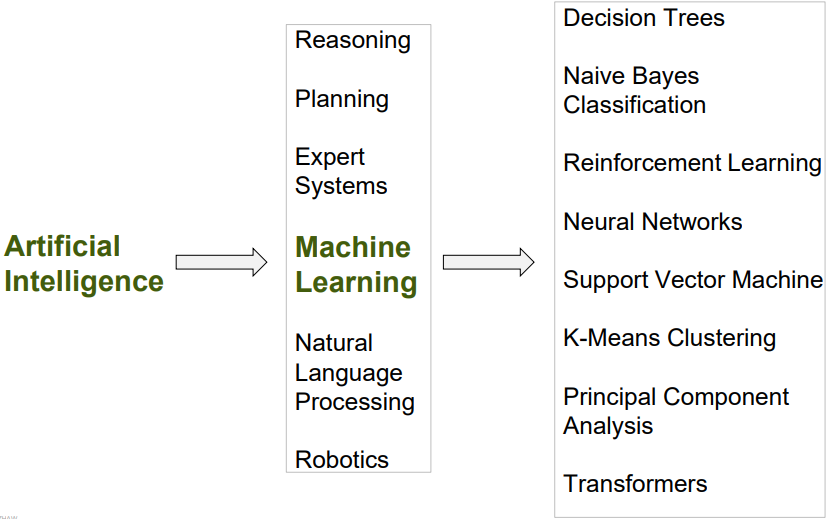
\includegraphics[width=\linewidth]{AI_magic.png}
\end{definition}

\begin{definition}{Model}\\
A model is a logical, mathematical or probabilistic relationship between several variables.
\end{definition}

\begin{definition}{Learning (Training)}\\
Machine Learning employs adaptive models, which are configured and parameterized automatically based on the training data.
\end{definition}

\begin{theorem}{Overview of important Concepts}\\
    \textcolor{frog}{\textbf{Data Mining}}
    \begin{itemize}
        \item Discovering patterns in large data sets
        \item Extraction of patterns and knowledge from large amounts of data
    \end{itemize}
    \textcolor{frog}{\textbf{Deep Learning}}
    \begin{itemize}
        \item Subset of machine learning where artificial neural networks (\textcolor{frog}{\textbf{Deep Neural Networks}}), algorithms inspired by the human brain, learn from large amounts of data
        \item Uses multiple layers to progressively extract higher level features (attributes) from the raw input
    \end{itemize}
    \textcolor{frog}{\textbf{Reinforcement Learning}} (Trial and Error)
    \begin{itemize}
        \item Concerned with how software agents take actions in an environment in order to maximize some notion of cumulative reward
    \end{itemize}
\end{theorem}

\begin{concept}{Supervised vs. Unsupervised Learning}\\
    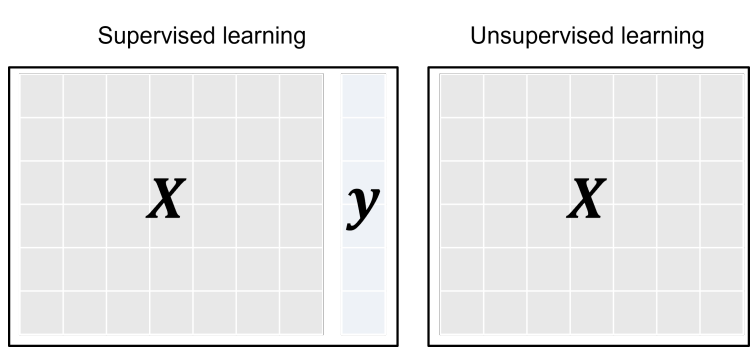
\includegraphics[width=\linewidth]{supervised_vs_unsupervised.png}
\end{concept}

\raggedcolumns

\multend

\begin{concept}{Overview of Machine Learning}\\
    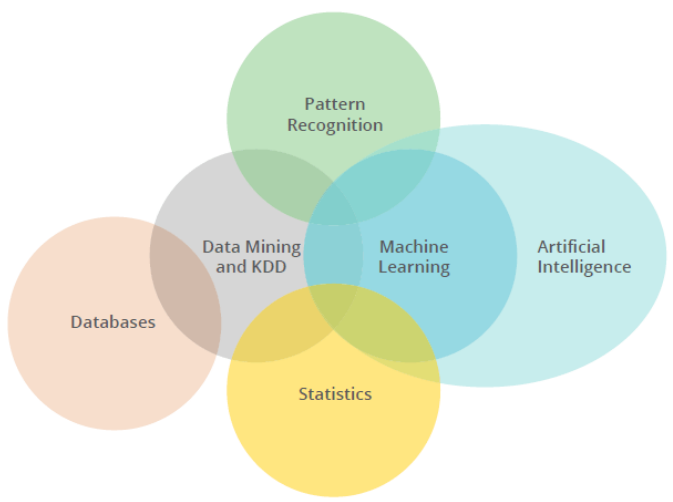
\includegraphics[width=0.55\linewidth]{intro_overview.png}
\end{concept}

\columnbreak

\subsection{Machine Learning Paradigms}

\begin{concept}{Supervised Learning}\\
    In Supervised Learning, we use a dataset with annotated training samples to 'teach' a machine to perform a certain task. The training data consists of pairs of inputs and their associated output values.
    \begin{itemize}
        \item The goal is to find a function $f$ that maps input data to their corresponding outputs.
        \item Input features are also called Independent Variables, Predictors, Attributes, or Covariates.
        \item The algorithm learns from labeled training data, and makes predictions (class, value) on unseen data
        \item Example: Classification, Regression (see script for math shit)
    \end{itemize}

    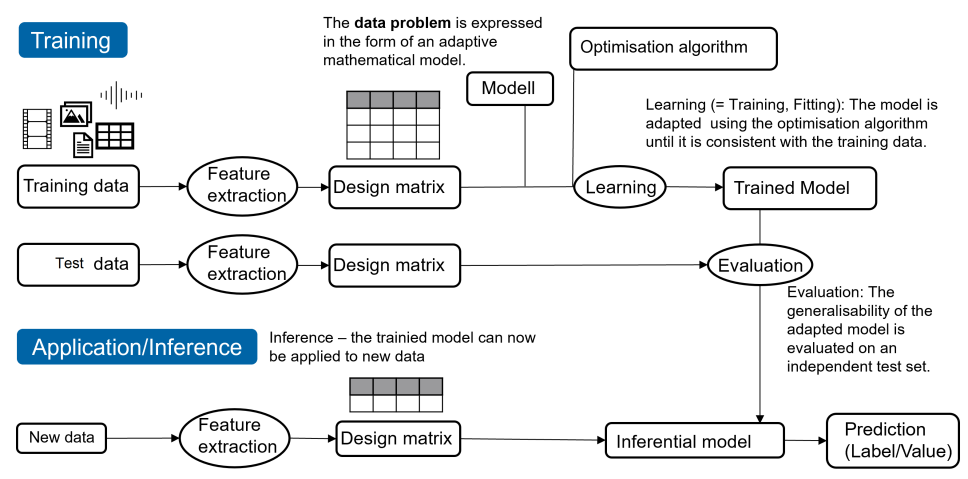
\includegraphics[width=\linewidth]{supervised_learning_pipeline.png}
\end{concept}

\begin{concept}{Unsupervised Learning}\\
    In Unsupervised Learning, the training data does not contain any expected output values. The goal is to model the underlying distribution of the data to explain it and apply the model to new data.
    \begin{itemize}
        \item The problem statement is fuzzier than in supervised learning
        \item Evaluation is more difficult without test data including expected output values
        \item The algorithm learns from unlabeled data, and determines data patterns / groupings / clusters
    \end{itemize}

    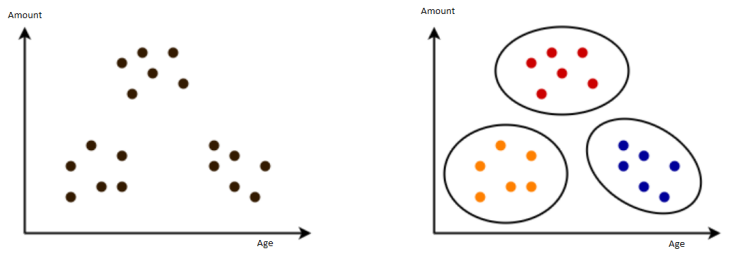
\includegraphics[width=0.8\linewidth]{clustering_data.png}
\end{concept}

\begin{concept}{Reinforcement Learning}

    \begin{minipage}{0.6\linewidth}
    In Reinforcement Learning, the learning system (called an Agent) can observe the Environment, select and perform Actions, and get Rewards in return. It must learn by itself what is the best strategy (called a Policy) to get the most reward over time.
    \begin{itemize}
        \item The algorithm learns to perform an action from experience
        \item Example: Game playing, Robotics
    \end{itemize}
    \end{minipage}
    \begin{minipage}{0.38\linewidth}
    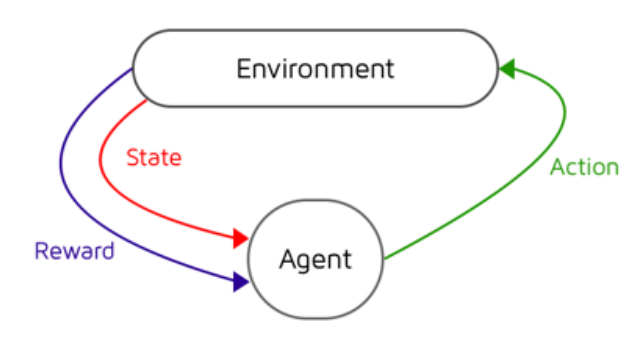
\includegraphics[width=\linewidth]{reinforcement_learning.png}
    \end{minipage}
\end{concept}

\subsubsection{Supervised Learning Details}

\mult{2}

\begin{definition}{Clustering}
    is the task of grouping a set of objects in such a way that objects in the same group (called a cluster) are more similar (in some sense) to each other than to
    those in other groups.
\end{definition}

\begin{definition}{Classification}
    is the problem of identifying to which of a set of categories a new observation belongs, on the basis of a training set of data containing observations (or instances) whose category membership is known. 
    E.g. correctly classifying (assigning a label to) an email as spam or not spam.

    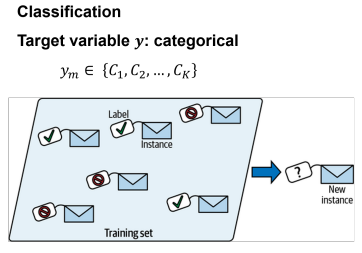
\includegraphics[width=\linewidth]{classification.png}
\end{definition}

\begin{definition}{Regression}
    is the problem of predicting and forecasting a concrete number based on a set of data containing observations whose category is known.

    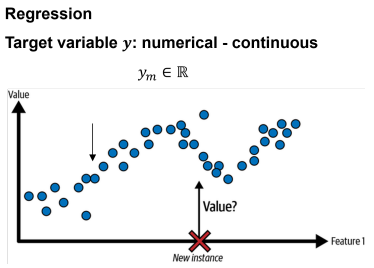
\includegraphics[width=\linewidth]{regression.png}
\end{definition}

\raggedcolumns


\begin{definition}{Classification vs. Regression}
\begin{itemize}
    \item \textbf{Classification}: The target variable is categorical (typically nominal scale). 
    The output values belong to a set of discrete classes $$y^{(m)} \in \{C_1, C_2, \ldots, C_K\}$$ 
    \\ Example: Spam filter classifying emails as 'spam' or 'not spam'.
    \vspace{-2mm}\\
    \item \textbf{Regression}: The target variable is a numeric (continuous) value: $$y^{(m)} \in \mathbb{R}$$
    \\ Example: Predicting the price of a car from features like mileage, age, brand, etc.
\end{itemize}
\end{definition}

\begin{definition}{Evaluating Supervised ML Models}\\
We typically estimate model performance by measuring the quality on a Testset, which contains data samples not used during training.
\begin{itemize}
    \item The data is split into Training set and Testset
    \item The model is trained on the training set and evaluated on the testset
    \item For regression, we use metrics like Mean Squared Error
    \item For classification, we use metrics like Accuracy, Precision, and Recall
\end{itemize}
\end{definition}

\begin{concept}{Supervised Learning Pipeline}\\
A typical supervised learning pipeline includes:
\begin{enumerate}
    \item Computing features for the samples (creating the Design Matrix)
    \item Selecting and training a machine learning algorithm/model
    \item Evaluating model performance on a test set
    \item Applying the final model to predict outcomes for new data
\end{enumerate}
This process is typically iterated several times to improve model quality.
\end{concept}

\multend

\begin{KR}{Building a Supervised Learning Model}
\paragraph{Define the problem}
Clearly specify what you want to predict and what data you have available.

\paragraph{Prepare the data}
\begin{itemize}
    \item Collect relevant data
    \item Clean the data (handle missing values, outliers)
    \item Split into training, validation, and test sets (e.g., 70\%, 15\%, 15\%)
\end{itemize}

\paragraph{Feature engineering}
\begin{itemize}
    \item Select relevant features
    \item Transform features if needed (normalization, encoding categorical variables)
    \item Create new features if beneficial
\end{itemize}

\paragraph{Model selection and training}
\begin{itemize}
    \item Choose appropriate algorithms based on the problem
    \item Train models with different hyperparameters
    \item Evaluate on validation set and tune hyperparameters
\end{itemize}

\paragraph{Final evaluation and deployment}
\begin{itemize}
    \item Evaluate final model on test set
    \item Deploy model for making predictions on new data
    \item Monitor performance and retrain periodically if needed
\end{itemize}
\end{KR}

\begin{example2}{Supervised Learning Example}
Consider a spam filter:
\begin{itemize}
    \item Input: Email text (converted to features like word frequencies)
    \item Output: Binary classification (spam or not spam)
    \item Training: The model learns patterns from labeled emails
    \item Inference: New emails are classified based on learned patterns
    \item Evaluation: Accuracy might be 98\% (98 out of 100 emails correctly classified)
\end{itemize}
\end{example2}


